\documentclass[11pt,a4paper]{article}

% Compiled with XeLaTeX (tectonic). Against the preamble originally proposed, the lines
% meant for pdflatex are replaced by their Unicode equivalents:
%   fontenc T1 + inputenc utf8  -> dropped: XeTeX does not need them
%   newtxmath[libertine]        -> unicode-math with Libertinus Math
%   beramono                    -> DejaVu Sans Mono, the same design as Bera (Vera) Mono
%                                  but with Lean code's Unicode symbols
% The theorem definitions come after cleveref: before it, \cref calls lemmas and
% remarks "theorem" as well.

% --- fonts and encoding ----------------------------------------------
\usepackage{libertine}                          % testo: Linux Libertine (OpenType)
\setmonofont{DejaVuSansMono.ttf}[Scale=0.85,    % codice: DejaVu Sans Mono,
  BoldFont=DejaVuSansMono-Bold.ttf,               % dritto anche dentro il corsivo
  ItalicFont=DejaVuSansMono.ttf]
% DejaVu Sans Mono has no ∣ (U+2223): that one character comes from Noto Sans Mono
\newfontfamily\leanfallbackfont{NotoSansMono-Regular.ttf}[Scale=0.85]

% --- page layout -----------------------------------------------------
\usepackage[a4paper,margin=1.1in,footskip=0.5in]{geometry}
\linespread{1.06}
\setlength{\parskip}{0pt}
\usepackage{microtype}
\setlength{\emergencystretch}{3em}
\usepackage{needspace}                          % titoli e listati brevi non separati

% --- mathematics -----------------------------------------------------
\usepackage{amsmath,amssymb,amsthm,mathtools}
\usepackage{unicode-math}
\setmathfont{LibertinusMath-Regular.otf}        % matematica coordinata con Libertine
\medmuskip=4mu plus 2mu minus 2mu               % gli spazi intorno a + e - non si annullano

% --- headings --------------------------------------------------------
\usepackage[explicit]{titlesec}
\titleformat{\section}{\normalfont\large\bfseries}{\thesection}{0.7em}{#1}
\titleformat{\subsection}{\normalfont\bfseries}{\thesubsection}{0.7em}{#1}
\titlespacing*{\section}{0pt}{1.6\baselineskip}{0.6\baselineskip}

% --- code ------------------------------------------------------------
\usepackage{xcolor}
\definecolor{rulecol}{gray}{0.75}
\definecolor{codebg}{gray}{0.975}
\usepackage{listings}
\lstset{
  basicstyle=\ttfamily\small,
  backgroundcolor=\color{codebg},
  frame=leftline, framerule=0.8pt, rulecolor=\color{rulecol},
  framexleftmargin=6pt, xleftmargin=8pt,
  breaklines=true, breakatwhitespace=true,
  showstringspaces=false, columns=fullflexible,
  keepspaces=true, upquote=true,
  aboveskip=0.9\baselineskip, belowskip=0.9\baselineskip,
}
% Line-break mark: without it a wrapped line looks like a new line at a different
% indentation, and in Lean indentation means something.
\lstset{extendedchars=true, postbreak=\mbox{$\hookrightarrow$}\space}
\lstdefinestyle{inline}{basicstyle=\ttfamily, frame=none, breaklines=false}
\newcommand{\li}{\lstinline[style=inline]}
% With XeTeX, listings passes only characters below 256 through its buffer; the rest
% are printed as soon as they are read, before the pending word ("⟨m, rfl⟩" came out
% as "⟨m, ⟩rfl"). Here the non-ASCII characters of the Lean files are registered the
% way listings registers the 8-bit ones.
\makeatletter
\def\leanchar#1#2{\catcode`#2=\active\lccode`\~=`#2\lccode`\/=`#2\lowercase{\def~{#1/}}}
\def\leandivides{{\leanfallbackfont ∣}}
\lst@AddToHook{SelectCharTable}{%
  \leanchar\lst@ProcessLetter κ\leanchar\lst@ProcessLetter ℕ\leanchar\lst@ProcessLetter ℤ%
  \leanchar\lst@ProcessOther ⟨\leanchar\lst@ProcessOther ⟩\leanchar\lst@ProcessOther ∀%
  \leanchar\lst@ProcessOther ∃\leanchar\lst@ProcessOther −\leanchar\lst@ProcessOther ∧%
  \leanchar\lst@ProcessOther ≠\leanchar\lst@ProcessOther ≡\leanchar\lst@ProcessOther ≤%
  \leanchar\lst@ProcessOther ≥\leanchar\lst@ProcessOther →\leanchar\lst@ProcessOther ←%
  \leanchar\lst@ProcessOther ↔%
  \catcode`∣=\active\lccode`\~=`∣\lowercase{\def~{\lst@ProcessOther\leandivides}}}
\makeatother

% --- tables, figures, references -------------------------------------
\usepackage{booktabs}
\usepackage{tikz}
\usetikzlibrary{decorations.pathreplacing}      % la graffa della figura
\usepackage[font=small,labelfont=bf]{caption}
\usepackage[hidelinks]{hyperref}
\usepackage{cleveref}

% --- theorems (after cleveref) ---------------------------------------
\theoremstyle{plain}
\newtheorem{theorem}{Theorem}
\newtheorem{lemma}[theorem]{Lemma}
\theoremstyle{remark}
\newtheorem{remark}[theorem]{Remark}

% --- footer ----------------------------------------------------------
\usepackage{fancyhdr}
\pagestyle{fancy}\fancyhf{}
\fancyfoot[C]{\thepage}
\renewcommand{\headrulewidth}{0pt}

% --- values taken from the verification report; files attached to the PDF ---
\input{build/values.tex}
\newcommand{\attachsource}[2]{%
  \special{pdf:fstream @#1 (lean/#2) << /Type /EmbeddedFile >>}%
  \special{pdf:names /EmbeddedFiles (#2)
    << /Type /Filespec /F (#2) /UF (#2) /EF << /F @#1 >> >>}}

\title{OEIS A105020 and the binary Goldbach conjecture:\\
an elementary equivalence and its Lean~4 formalization}
\author{Federico Di Candia}
\date{12 September 2026}

\begin{document}
\maketitle
\attachsource{solution}{Solution.lean}%
\attachsource{challenge}{Challenge.lean}%
\attachsource{config}{config.json}%
\attachsource{meaning}{MeaningChecks.lean}%

\begin{abstract}
The formal-conjectures repository contains \li{OeisA105020.conjecture}, a Lean
formalization of a 2007 comment on OEIS A105020 that presents it as ``a Goldbach
Conjecture for this sequence''. We give an elementary proof that this formal statement
is equivalent to the repository's statement of the binary Goldbach conjecture,
including an index lemma needed because the formal statement quantifies over arbitrary
indices, and a Lean~4 formalization of every result stated here, checked with
comparator. No novelty is claimed for the mathematical content: the underlying
correspondence is implicit in a 2021 formula of W.~I.~Hurt in OEIS A045917
(Section~\ref{sec:prior}).
\end{abstract}

\section{Introduction}\label{sec:intro}

The formal-conjectures repository~\cite{fc} collects open conjectures stated in
Lean~4 with Mathlib~\cite{mathlib}, each tagged with its status. One of them,
\li{OeisA105020.conjecture}, formalizes a comment added in 2007 by M.~Hiebl to OEIS
A105020~\cite{oeis-a105020}, which presents it as ``a Goldbach Conjecture for this
sequence''; the repository marks it as an open research problem. The sequence lists
the differences of squares $m^2 - n^2$ with $m > n$, arranged in an array and read by
antidiagonals. The comment asserts that for $n \ge 1$, whenever two odd terms $2n+1$
and $2n+3$ occur with exactly $n$ terms between them, at least one of those terms is a
semiprime, that is, a product of two primes, not necessarily distinct.

The name is apt. On antidiagonal $n$ the term at offset $k$ factors as
$(k+1)(2n+1-k)$, a product of two integers whose sum is $2n+2$ for every $k$
(Figure~\ref{fig:antidiagonal}). A product $pq$ with $p, q \ge 2$ is a semiprime exactly
when $p$ and $q$ are both prime, so the semiprimes strictly between the first term
$2n+1$ of antidiagonal $n$ and the first term $2n+3$ of antidiagonal $n+1$ correspond
to the ways of writing $2n+2$ as a sum of two primes. This correspondence is not new:
it underlies a 2021 formula of W.~I.~Hurt in OEIS A045917, discussed in
Section~\ref{sec:prior}.

The formal statement, however, does not mention antidiagonals. It quantifies over all
indices $i$ and $j$ with $a(i) = 2n+1$, $a(j) = 2n+3$ and $j = i+n+1$, and odd values
occur in A105020 at many positions other than the start of an antidiagonal
(Remark~\ref{rem:values}). The correspondence alone therefore shows only that the
formal statement implies Goldbach. The converse needs the fact that these hypotheses
force $i$ and $j$ to be the first indices of antidiagonals $n$ and $n+1$. This is
Lemma~\ref{lem:index}, an elementary computation with the closed form of the terms.
With it, \li{OeisA105020.conjecture} is equivalent to the repository's own statement of
the binary Goldbach conjecture (Theorem~\ref{thm:main}), so a proof or a
counterexample for either would settle the other.

Every result stated in Sections~\ref{sec:indices}--\ref{sec:equiv} is formalized in Lean
and checked with comparator~\cite{comparator}, which certifies that a solution proves
exactly the statements of a challenge file and uses only standard axioms. That
guarantee is only as good as the challenge file, so we also check separately that its
statements mean what this note says: that both repository statements elaborate to the
expected propositions, that the Goldbach side does not depend on \li{sorryAx}, and that
the definitions agree with the OEIS data. Independently of the proofs, an exhaustive
search found no index pair other than the canonical ones among all $i < 10^{10}$.

Section~\ref{sec:defs} recalls the definitions and the two statements.
Section~\ref{sec:indices} describes the indices of A105020 and the closed form of its
terms, Section~\ref{sec:lemma} proves the index lemma, and Section~\ref{sec:equiv}
proves the equivalence. Section~\ref{sec:lean} describes the formalization, its
verification and the meaning checks, and Section~\ref{sec:prior} discusses prior work
and what this note adds. Appendix~\ref{app:quoted} quotes the repository statements
and Hurt's formula, Appendix~\ref{app:repro} explains how to reproduce the
verification, and Appendices~\ref{app:solution}--\ref{app:meaning} contain the Lean
files, which are also attached to this PDF.

\section{Definitions and statements}\label{sec:defs}

Throughout, $T_c = c(c+1)/2$. The sequence A105020~\cite{oeis-a105020} is the array
whose row $n \ge 0$ contains the numbers $m^2 - n^2$ for $m \ge n+1$, read by upward
antidiagonals. The repository~\cite{fc} defines it in the file
\nolinkurl{FormalConjectures/OEIS/105020.lean}, quoted in Appendix~\ref{app:defs}.
With \li{triangularNumber c}, which is $\binom{c+1}{2} = T_c$, and
\[
  \operatorname{antidiagonalIndex}(N)
    = \bigl\lfloor (\lfloor \sqrt{8N+1} \rfloor - 1)/2 \bigr\rfloor,
\]
the definition reads
\[
  a(N) = (c+1)^2 - (c-k)^2, \qquad \text{where } c = \operatorname{antidiagonalIndex}(N)
  \text{ and } k = N - T_c,
\]
with all operations on $\mathbb{N}$ and truncated subtraction. Thus $a$ is indexed
from $0$, with $a(0) = 1$. This agrees with the current offset of the OEIS entry, whose
b-file also starts at $a(0) = 1$.

The comment on A105020 reads:
\begin{quote}
A ``Goldbach Conjecture'' for this sequence: when there are n terms between
consecutive odd integers (2n+1) and (2n+3) for n > 0, at least one will be the product
of 2 primes (not necessarily distinct). --- M.~Hiebl, Jul 15 2007
\end{quote}
The comment continues with an example for $n = 3$ that names $a(7) = 7$ and
$a(11) = 9$, with the intermediate terms $a(8) = 12$, $a(9) = 15$ and $a(10) = 16$.
These indices are shifted by one with respect to the entry's current offset: in the
b-file, and in the repository's $a$, the same terms are $a(6), \dots, a(10)$. The
formal statement below involves only values and differences of indices, so the shift
does not affect it (a machine check is in Appendix~\ref{app:meaning}).

The repository formalizes the comment as \li{OeisA105020.conjecture}
(Appendix~\ref{app:conj}). It states that for all $n, i, j \in \mathbb{N}$,
\[
\begin{aligned}
  &n \ge 1,\quad a(i) = 2n+1,\quad a(j) = 2n+3,\quad j = i+n+1\\
  &\qquad \implies \text{there is } k \in \mathbb{N} \text{ with } i < k < j
    \text{ and } a(k) \text{ a semiprime.}
\end{aligned}
\]
Here \li{Nat.IsSemiprime m} is Mathlib's \li{Nat.IsAlmostPrime 2 m}, that is,
$m \neq 0$ and $\Omega(m) = 2$, where $\Omega(m)$ is the number of prime factors of $m$
counted with multiplicity.

The binary Goldbach conjecture is \li{GoldbachConjecture.goldbach}, in
\nolinkurl{FormalConjectures/Wikipedia/GoldbachConjecture.lean}
(Appendix~\ref{app:goldbach}):
\[
\begin{aligned}
  \texttt{answer(sorry)} \iff{}
    &\text{for all } n \in \mathbb{N} \text{ with } n > 2 \text{ and } n \text{ even},\\
    &\text{there are primes } p, q \text{ with } n = p + q.
\end{aligned}
\]
With the repository's default option, \li{answer(sorry)} elaborates to \li{True}. This,
and the exact elaborated form of both statements, is checked in
Section~\ref{sec:meaning}; Appendix~\ref{app:repro} describes a build-configuration
caveat.

\section{Indices on antidiagonals}\label{sec:indices}

\begin{lemma}[Index decomposition]\label{lem:decomp}
Every $N \ge 0$ can be written in exactly one way as $N = T_c + k$ with
$0 \le k \le c$. Moreover, if $N = T_c + k$ with $0 \le k \le c$, then $c$ is
$\operatorname{antidiagonalIndex}(N)$.
\end{lemma}

\begin{proof}
Let $t = \lfloor \sqrt{8N+1} \rfloor$ and $c = \lfloor (t-1)/2 \rfloor$, so that
$2c+1 \le t \le 2c+2$. From $8T_c + 1 = (2c+1)^2 \le t^2 \le 8N+1$ we get
$T_c \le N$, and from $8N+1 < (t+1)^2 \le (2c+3)^2 = 8T_{c+1} + 1$ we get
$N < T_{c+1} = T_c + c + 1$. Conversely, if $N = T_c + k$ with $0 \le k \le c$, then
\[
  (2c+1)^2 \le 8N+1 = (2c+1)^2 + 8k < (2c+3)^2,
\]
so $\lfloor \sqrt{8N+1} \rfloor \in \{2c+1,\, 2c+2\}$ and therefore
$\lfloor (\lfloor \sqrt{8N+1} \rfloor - 1)/2 \rfloor = c$, which is
$\operatorname{antidiagonalIndex}(N)$. In particular $c$, and hence $k = N - T_c$, is
determined by $N$.
\end{proof}

\begin{lemma}[Closed form]\label{lem:closed}
For $0 \le k \le c$,
\[
  a(T_c + k) = (c+1)^2 - (c-k)^2 = (k+1)(2c+1-k).
\]
With $s = c+1$ and $d = k+1$ this reads $a(T_c + k) = d\,(2s-d)$. In particular
$a(T_n) = 2n+1$ for every $n \ge 0$.
\end{lemma}

\begin{proof}
By Lemma~\ref{lem:decomp} the antidiagonal index of $T_c + k$ is $c$, so the
definition of $a$ uses $c$ and $k$. Since $k \le c < c+1$, none of the subtractions on
$\mathbb{N}$ truncates, and
\[
  a(T_c + k) = (c+1)^2 - (c-k)^2 = (k+1)(2c+1-k).
\]
Taking $k = 0$ gives $a(T_n) = 2n+1$.
\end{proof}

\begin{remark}[Values and factorizations]\label{rem:values}
The indices at which $a$ takes a given value $v$ correspond to the factorizations of
$v$: $a(N) = v$ if and only if there are integers $d, e$ with $1 \le d \le e$,
$d \equiv e \pmod 2$ and $v = de$, such that $N = T_{(d+e)/2-1} + (d-1)$. Different
such factorizations give different indices, by the uniqueness in
Lemma~\ref{lem:decomp}. In particular an odd value occurs once for every factorization
into two factors $d \le e$, and not only at the start of an antidiagonal.
\end{remark}

\begin{figure}[t]
\centering
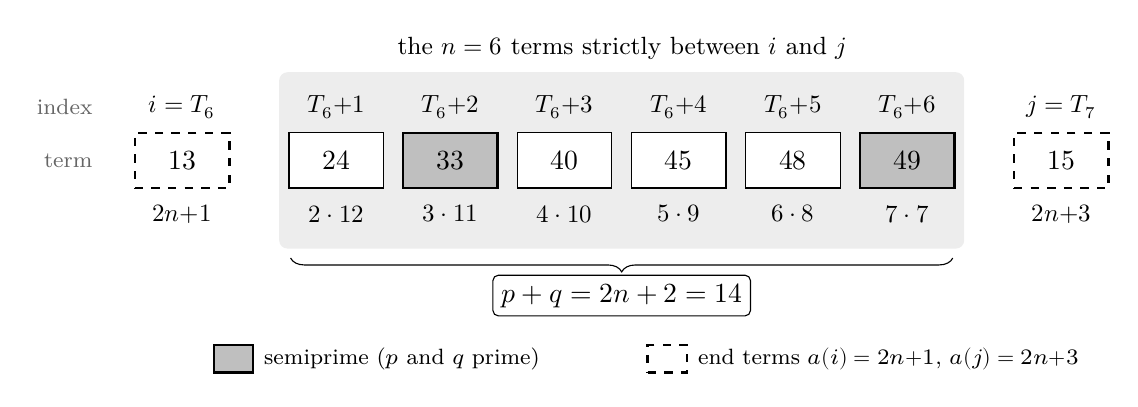
\begin{tikzpicture}[x=14.5mm, y=8mm,
    term/.style={draw, fill=white, minimum width=12mm, minimum height=7mm, inner sep=0pt},
    semi/.style={term, fill=black!25, line width=0.9pt},
    endterm/.style={term, dashed, line width=0.9pt},
    idx/.style={font=\small},
    note/.style={font=\footnotesize, text=black!60}]
  % the n terms strictly between i and j: the only ones the conjecture looks at
  \fill[black!7, rounded corners=3pt] (0.5,-1.4) rectangle (6.5,1.4);
  \node[font=\small, anchor=south] at (3.5,1.45)
    {the $n = 6$ terms strictly between $i$ and $j$};
  \foreach \k/\v/\p/\q/\st in {1/24/2/12/term, 2/33/3/11/semi, 3/40/4/10/term,
                               4/45/5/9/term, 5/48/6/8/term, 6/49/7/7/semi} {
    \node[\st] at (\k,0) {$\v$};
    \node[idx] at (\k,0.85) {$T_6{+}\k$};
    \node[idx] at (\k,-0.85) {$\p\cdot\q$};
  }
  % the two odd end terms, outside the range
  \node[endterm] at (-0.35,0) {$13$};
  \node[endterm] at (7.35,0) {$15$};
  \node[idx] at (-0.35,0.85) {$i = T_6$};
  \node[idx] at (7.35,0.85) {$j = T_7$};
  \node[idx] at (-0.35,-0.85) {$2n{+}1$};
  \node[idx] at (7.35,-0.85) {$2n{+}3$};
  % row labels
  \node[note, anchor=east] at (-1.05,0.85) {index};
  \node[note, anchor=east] at (-1.05,0) {term};
  % the constant sum
  \draw[decorate, decoration={brace, mirror, amplitude=5pt}]
    (0.6,-1.55) -- (6.4,-1.55)
    node[midway, below=6pt, draw, rounded corners=2pt, inner sep=3pt]
      {$p + q = 2n+2 = 14$};
  % legend
  \node[semi, minimum width=5mm, minimum height=3.5mm] (l1) at (0.1,-3.15) {};
  \node[font=\footnotesize, anchor=west] at (l1.east) {semiprime ($p$ and $q$ prime)};
  \node[endterm, minimum width=5mm, minimum height=3.5mm] (l2) at (3.9,-3.15) {};
  \node[font=\footnotesize, anchor=west] at (l2.east)
    {end terms $a(i) = 2n{+}1$, $a(j) = 2n{+}3$};
\end{tikzpicture}
\caption{Antidiagonal $n = 6$ of A105020 (indices $T_6 = 21$ to $T_6 + 6 = 27$) and the
first term of antidiagonal $7$ ($T_7 = 28$). By Lemma~\ref{lem:closed} the term at
$T_6 + k$ is $pq$ with $p = k+1$ and $q = 2n+1-k$. The end terms $13$ and $15$ play
the roles of $a(i)$ and $a(j)$ in the conjecture and are not among the terms it looks
at, so $15 = 3 \cdot 5$ does not count. The semiprimes among the $n$ terms between
them, $33 = 3 \cdot 11$ and $49 = 7 \cdot 7$, correspond to the Goldbach partitions
$14 = 3 + 11 = 7 + 7$.}
\label{fig:antidiagonal}
\end{figure}

\section{The index lemma}\label{sec:lemma}

\begin{lemma}[Index lemma]\label{lem:index}
Let $n \ge 1$, and suppose that $a(i) = 2n+1$, $a(j) = 2n+3$ and $j = i+n+1$. Then
$i = T_n$ and $j = T_{n+1}$.
\end{lemma}

\begin{proof}
Put $u = 2n+1$. By Lemma~\ref{lem:decomp}, write $i = T_s - 1 - r$ with $s \ge 1$ and
$0 \le r \le s-1$ (in the notation of Lemma~\ref{lem:decomp}, $s = c+1$ and
$r = c-k$), and put $d = s-r$, so that $1 \le d \le s$. Similarly, write
$j = T_{s'} - 1 - r'$ and put $d' = s' - r' \ge 1$. By Lemma~\ref{lem:closed},
\[
  u = s^2 - r^2 = d\,(2s-d), \qquad u + 2 = s'^2 - r'^2 = d'\,(2r'+d').
\]
Since $3 \le u \le s^2$, we have $s \ge 2$.

\emph{Step 1.} Expanding with $s = r+d$ and $s' = r'+d'$ gives the polynomial identity
\[
  2(j-i) - (u+1) = \bigl[\, r'(r'-1) + d' - s(s-1) - 2d + 1 \,\bigr]
    + \bigl[\, d'(2r'+d') - d(2s-d) - 2 \,\bigr].
\]
The second bracket vanishes because $a(j) = u+2$, and the left-hand side vanishes
because $j - i = (u+1)/2$. Hence
\begin{align}
  r'(r'-1) + d' &= s(s-1) + 2d - 1, \tag{F}\label{eq:F}\\
  d'(2r'+d') &= d(2s-d) + 2. \tag{E}\label{eq:E}
\end{align}

\emph{Step 2.} Let $\varepsilon = 2d - 1 - d'$, so that \eqref{eq:F} reads
$r'(r'-1) = s(s-1) + \varepsilon$.

\emph{Case $\varepsilon \ge 0$.} Since $d \le s$ and $d' \ge 1$, we have
$\varepsilon \le 2s-2$, hence $s(s-1) \le r'(r'-1) < s(s+1)$. As $s(s-1) \ge 2$, this
forces $r' \ge 2$; the map $x \mapsto x(x-1)$ is strictly increasing on the integers
$x \ge 1$, so $r' = s$ and $\varepsilon = 0$, that is, $d' = 2d-1$. Substituting in
\eqref{eq:E},
\[
  (2d-1)(2s+2d-1) - d(2s-d) - 2 = (d-1)(2s+5d+1) = 0,
\]
so $d = 1$. Then $r = s-1$ and $u = 2s-1$, so $s = n+1$ and
$i = T_{n+1} - 1 - n = T_n$; finally $j = T_n + n + 1 = T_{n+1}$.

\emph{Case $\varepsilon < 0$.} Then $r'(r'-1) < s(s-1)$, so $r' \le s-1$ and
$r'(r'-1) \le (s-1)(s-2)$. By \eqref{eq:F},
\[
  d' = s(s-1) + 2d - 1 - r'(r'-1) \ge 2(s-1) + 2d - 1 \ge 2s - 1.
\]
On the other hand, by \eqref{eq:E},
$d'^2 \le d'(2r'+d') = s^2 - r^2 + 2 \le s^2 + 2 < (s+1)^2$, so $d' \le s$. Hence
$2s - 1 \le s$, that is, $s \le 1$, a contradiction.
\end{proof}

\section{The equivalence}\label{sec:equiv}

\begin{theorem}\label{thm:main}
\li{OeisA105020.conjecture} holds if and only if every even integer greater than $2$
is the sum of two primes.
\end{theorem}

\begin{proof}
Let $n \ge 1$. The indices $i = T_n$ and $j = T_{n+1}$ satisfy the hypotheses of the
conjecture: $a(T_n) = 2n+1$ and $a(T_{n+1}) = 2n+3$ by Lemma~\ref{lem:closed}, and
$T_{n+1} = T_n + n + 1$. The indices strictly between them are $T_n + k$ with
$1 \le k \le n$, and by Lemma~\ref{lem:closed}
\[
  a(T_n + k) = (k+1)(2n+1-k) = pq, \qquad p = k+1, \quad q = 2n+1-k.
\]
Then $p + q = 2n+2$ and $p, q \ge 2$. Since $\Omega(pq) = \Omega(p) + \Omega(q)$ and
both terms are at least $1$, the number $pq$ is a semiprime if and only if $p$ and $q$
are both prime.

($\Rightarrow$) Let $m > 2$ be even, and write $m = 2n+2$ with $n \ge 1$. Applying the
conjecture to $(n, T_n, T_{n+1})$ gives an index strictly between $T_n$ and
$T_{n+1}$, that is, $T_n + k$ with $1 \le k \le n$, at which $a$ is a semiprime; hence
$m = p + q$ with $p$ and $q$ prime.

($\Leftarrow$) Let $(n, i, j)$ satisfy the hypotheses. By Lemma~\ref{lem:index},
$i = T_n$ and $j = T_{n+1}$. By Goldbach, $2n+2 = p + q$ with primes $p \le q$, so
$2 \le p \le n+1$. The index $T_n + (p-1)$ lies strictly between $i$ and $j$, and
$a(T_n + (p-1)) = p\,(2n+2-p) = pq$ is a semiprime.
\end{proof}

Without Lemma~\ref{lem:index} one obtains only that the formal statement implies
Goldbach. The formal statement quantifies over all pairs $(i,j)$ satisfying the
hypotheses, and Lemma~\ref{lem:index} is what yields the converse.

\section{Lean formalization and verification}\label{sec:lean}

\subsection{What is formalized}

The file \li{Solution.lean} (Appendix~\ref{app:solution}, \SolutionLines{} lines)
proves the \NumTheorems{} statements collected in \li{Challenge.lean}
(Appendix~\ref{app:challenge}), where each proof is \li{sorry}. Together they cover
every result stated in Sections~\ref{sec:indices}--\ref{sec:equiv} (all names are in
the namespace \li{A105020Goldbach}):

\begin{center}\small
\begin{tabular}{@{}p{0.30\textwidth}p{0.62\textwidth}@{}}
\toprule
Result & Lean statements \\
\midrule
Lemma~\ref{lem:decomp} & \texttt{exists\_index\_decomposition}\newline
  \texttt{index\_decomposition\_unique}\newline
  \texttt{antidiagonalIndex\_triangularNumber\_add} \\
Lemma~\ref{lem:closed} & \texttt{a\_triangularNumber\_add}\newline
  \texttt{a\_eq\_d\_mul}\newline
  \texttt{a\_triangularNumber} \\
Remark~\ref{rem:values} & \texttt{a\_eq\_iff\_exists\_factorization} \\
Lemma~\ref{lem:index} & \texttt{hypotheses\_force\_canonical\_indices} \\
Theorem~\ref{thm:main} & \texttt{conjecture\_iff\_goldbach} \\
\bottomrule
\end{tabular}
\end{center}

The definitions are the repository's own, and the two conjectures enter the last
statement only through \li{type_of%}, so neither is restated:
\li{conjecture_iff_goldbach} asserts that the type of \li{OeisA105020.conjecture} is
equivalent to the type of \li{GoldbachConjecture.goldbach}. The latter type is
\li{True ↔ P}, where \li{P} is the Goldbach statement, so the theorem says that
\li{OeisA105020.conjecture} is equivalent to \li{True ↔ P}, and hence to \li{P}.

\subsection{Verification}\label{sec:verification}

The formalization was checked with comparator~\cite{comparator}, configured as in
Appendix~\ref{app:config}. For each listed theorem, comparator guarantees that the
solution module (i)~proves the same elaborated statement as the challenge module,
(ii)~uses no axioms beyond \li{propext}, \li{Classical.choice} and \li{Quot.sound},
and (iii)~is accepted by the Lean kernel.

\medskip
\noindent\textbf{Result.} \li{Your solution is okay!} for all \NumTheorems{} theorems
(\VerifySeconds~s).
\medskip

\begin{center}\small
\begin{tabular}{@{}lp{0.68\textwidth}@{}}
\toprule
Component & Version \\
\midrule
formal-conjectures & commit \texttt{0a8b856c01b3911c52174ea4d0944097bd398bf7} (2026-09-10), with
  the \texttt{lakefile.toml} change described in Appendix~\ref{app:repro} \\
Lean & v4.33.1 \\
Mathlib & commit \texttt{0df444a360eaa60ab8c11dca51a86af692955474} (tag v4.33.1) \\
comparator & commit \texttt{2312244ac716564a61cc0bf4e107d9abf1757a61} (2026-08-30) \\
lean4export & commit \texttt{411dce7db58a3afc60ecab2d211acd1042b593dc} (2026-08-25) \\
Platform & macOS; \texttt{landrun} replaced by a non-sandboxing shim
  (Appendix~\ref{app:repro}) \\
\bottomrule
\end{tabular}
\end{center}

We ran comparator through a local wrapper that also performs a syntactic pre-check of
the solution (no \li{sorry}, \li{admit}, \li{axiom} or \li{native_decide}; imports
restricted to Mathlib and the two repository modules), runs the build under macOS
\texttt{sandbox-exec}, and checks that the repository files are unchanged after the
run. None of this is needed to reproduce the result; Appendix~\ref{app:repro} explains
how to do so.

\subsection{Meaning of the challenge}\label{sec:meaning}

comparator certifies that the solution proves exactly the statements of the challenge;
it does not certify that those statements mean what this note says. That is checked by
\li{MeaningChecks.lean} (Appendix~\ref{app:meaning}), which compiles against the same
repository using only standard axioms:
\begin{itemize}
\item Both repository statements elaborate, by \li{rfl}, to the forms quoted in
  Appendix~\ref{app:quoted}. In particular the Goldbach side is definitionally
  \li{True ↔ P} (and not \li{False ↔ P}), and \li{goldbach_statement_elaborates}
  depends only on \li{propext}: the elaborated statement contains no \li{sorryAx}.
\item \li{Prime}, \li{Even} and \li{Nat.IsSemiprime} have their usual meaning on
  $\mathbb{N}$.
\item \li{triangularNumber} agrees with $T_c$, and \li{a} agrees with the OEIS b-file
  for $a(0), \dots, a(11)$; the terms of Hiebl's example sit at the indices
  $6, \dots, 10$.
\item The hypotheses of Lemma~\ref{lem:index} are satisfiable ($n = 3$, $i = T_3$,
  $j = T_4$), so that statement is not vacuous.
\item Each challenge statement is restated as a proposition, generated from the text of
  \li{Challenge.lean}, and printed with full names, which shows that \li{a},
  \li{triangularNumber} and \li{antidiagonalIndex} resolve to the repository's
  constants in the namespace \li{OeisA105020}.
\end{itemize}

\subsection{Remarks}

\begin{itemize}
\item The formal proof follows Sections~\ref{sec:indices}--\ref{sec:equiv}. In
  Lemma~\ref{lem:index} it distinguishes the cases $r' < s$, $r' = s$ and $r' > s$
  instead of the sign of $\varepsilon$; the two case splits cover the same ground.
\item Nonlinear steps are discharged by \li{linear_combination} and \li{linarith} from
  explicitly stated polynomial identities, each checked by \li{ring}. No options such as
  \li{maxHeartbeats} are set.
\item As a sanity check independent of the proof, an exhaustive search found no index
  pair other than $(T_n, T_{n+1})$ satisfying the hypotheses of
  Lemma~\ref{lem:index}, among all $i < 10^{10}$ and among all non-canonical indices
  whose value is at most $4 \cdot 10^{9}$.
\end{itemize}

\section{Prior work, and what this note adds}\label{sec:prior}

\paragraph{The mathematical fact is not new.}
OEIS A045917~\cite{oeis-a045917}, the number of decompositions of $2n$ into unordered
sums of two primes, contains the formula
\[
  \mathrm{A045917}(n) = \sum_{k = n(n-1)/2 + 2}^{n(n+1)/2}
    \mathrm{A064911}\bigl(\mathrm{A105020}(k-1)\bigr)
\]
(W.~I.~Hurt, Sep 11 2021; Appendix~\ref{app:hurt} quotes it as written in the entry,
where $a(n)$ stands for $\mathrm{A045917}(n)$). Here A064911~\cite{oeis-a064911} is the
characteristic function of the semiprimes. The indices $k-1$ run over
$T_{n-1}+1, \dots, T_n - 1$, that is, over positions $1, \dots, n-1$ of antidiagonal
$n-1$ of A105020, which are the terms strictly between the odd terms $2n-1$ and $2n+1$.
The formula therefore says that the number of semiprimes strictly between these
consecutive odd terms equals the number of Goldbach partitions of $2n$, and the
equivalence of Hiebl's conjecture with Goldbach at the canonical indices follows at
once. We checked the formula numerically for $2 \le n \le 1500$. Two further entries by
the same author rest on the same correspondence: A228553~\cite{oeis-a228553} and
A350419~\cite{oeis-a350419}. The underlying identity
$(n+1)^2 - m^2 = (n+1-m)(n+1+m)$, which turns Goldbach partitions of $2n+2$ into
semiprimes written as differences of squares, is classical.

\paragraph{Not ours.}
The correspondence between semiprimes in A105020 and Goldbach partitions, and with it
the equivalence at the canonical indices.

\paragraph{What this note contributes.}
\begin{enumerate}
\item The observation that the repository's formal statement
  \li{OeisA105020.conjecture}, which quantifies over arbitrary indices, is equivalent
  to \li{GoldbachConjecture.goldbach}. This requires Lemma~\ref{lem:index}. We did
  not find Lemma~\ref{lem:index} written elsewhere; it is a routine computation, and we
  make no claim that it is new.
\item A Lean~4 formalization of every result stated in
  Sections~\ref{sec:indices}--\ref{sec:equiv}, checked with comparator, together with
  the meaning checks of Section~\ref{sec:meaning}.
\end{enumerate}

\paragraph{Provenance.}
The observation that \li{OeisA105020.conjecture} implies Goldbach was first produced
by an AI language model (Claude Opus~5, Anthropic) during an exploratory run on open
problems from formal-conjectures. The converse direction (Lemma~\ref{lem:index}), the
proofs in this note and the Lean formalization were produced in working sessions with
the same model under the author's direction, and were checked as described in
Section~\ref{sec:lean}. This note was drafted with AI assistance.

\begin{thebibliography}{9}
\raggedright
\bibitem{fc} Google DeepMind, \emph{formal-conjectures},
  \url{https://github.com/google-deepmind/formal-conjectures}, commit \texttt{0a8b856c}.
\bibitem{oeis-a105020} OEIS Foundation Inc., \emph{The On-Line Encyclopedia of Integer
  Sequences}, sequence A105020, \url{https://oeis.org/A105020}, accessed 12 September
  2026.
\bibitem{oeis-a045917} OEIS, sequence A045917, \url{https://oeis.org/A045917}.
\bibitem{comparator} \emph{comparator}, \url{https://github.com/leanprover/comparator},
  commit \texttt{2312244a}.
\bibitem{oeis-a064911} OEIS, sequence A064911, \url{https://oeis.org/A064911}.
\bibitem{oeis-a228553} OEIS, sequence A228553, \url{https://oeis.org/A228553}.
\bibitem{oeis-a350419} OEIS, sequence A350419, \url{https://oeis.org/A350419}.
\bibitem{mathlib} The mathlib Community, \emph{The Lean mathematical library},
  \url{https://github.com/leanprover-community/mathlib4}, commit \texttt{0df444a3}.
\end{thebibliography}

\clearpage
\appendix

\section{Quoted statements}\label{app:quoted}

The excerpts below are copied from the repository at the commit listed in
Section~\ref{sec:verification}, and from OEIS as accessed on 12 September 2026.

\subsection{Definitions of A105020}\label{app:defs}

From \nolinkurl{FormalConjectures/OEIS/105020.lean}, with the docstrings of the
last two definitions omitted:
\begin{lstlisting}
def triangularNumber (c : ℕ) : ℕ := Nat.choose (c + 1) 2

def antidiagonalIndex (n : ℕ) : ℕ :=
  (Nat.sqrt (8 * n + 1) - 1) / 2

def a (n : ℕ) : ℕ :=
  let c := antidiagonalIndex n
  let k := n - triangularNumber c
  let i := c - k
  let m := c + 1
  m^2 - i^2
\end{lstlisting}

\needspace{15\baselineskip}
\subsection{The formal conjecture}\label{app:conj}

From the same file:
\begin{lstlisting}
@[category research open, AMS 11]
theorem conjecture :
  ∀ (n i j : ℕ), 1 ≤ n →
    a i = 2 * n + 1 →
    a j = 2 * n + 3 →
    j = i + n + 1 →
    ∃ (k : ℕ),
      i < k ∧
      k < j ∧
      (a k).IsSemiprime := by
  sorry
\end{lstlisting}

\needspace{8\baselineskip}
\subsection{The binary Goldbach conjecture}\label{app:goldbach}

From \nolinkurl{FormalConjectures/Wikipedia/GoldbachConjecture.lean}:
\begin{lstlisting}[basicstyle=\ttfamily\footnotesize]
@[category research open, AMS 11]
theorem goldbach :
    answer(sorry) ↔ ∀ n : ℕ, 2 < n → Even n → ∃ p q, Prime p ∧ Prime q ∧ n = p + q := by
  sorry
\end{lstlisting}

\needspace{6\baselineskip}
\subsection{Hurt's formula in A045917}\label{app:hurt}

From the formula section of OEIS A045917~\cite{oeis-a045917}, where the line ends with
the attribution ``- Wesley Ivan Hurt, Sep 11 2021'':
\begin{lstlisting}
a(n) = Sum_{k=n*(n-1)/2+2..n*(n+1)/2} A064911(A105020(k-1)).
\end{lstlisting}

\section{Reproducing the verification}\label{app:repro}

The four files reproduced in Appendices~\ref{app:solution}--\ref{app:meaning} are
attached to this PDF as embedded files. Some PDF viewers, such as Adobe Acrobat Reader
and Firefox, list them in an attachments panel; \mbox{\texttt{pdfdetach -saveall}} (from
Poppler) extracts them. Use the attached files rather than text copied from the
appendices: copying from a PDF loses indentation, which is significant in Lean.

\needspace{8\baselineskip}
\subsection{Repository and build configuration}

Clone the repository at the commit used for the verification:
\begin{lstlisting}
git clone https://github.com/google-deepmind/formal-conjectures.git
cd formal-conjectures
git checkout 0a8b856c01b3911c52174ea4d0944097bd398bf7
\end{lstlisting}

\paragraph{Build-configuration caveat.}
At this commit \texttt{lakefile.toml} declares, besides the library
\texttt{FormalConjectures}, a second library \texttt{FormalConjecturesAnswerPostpone}
with the same glob and the option \li{google.answer = "postpone"}. The two libraries
write to the same build directory, so whether \li{answer(sorry)} elaborates to
\li{True} or to a \li{sorry} depends on which build command ran last. If
\li{GoldbachConjecture.goldbach} is built in \texttt{postpone} mode, its elaborated
type contains \li{sorryAx}, and the checks of Section~\ref{sec:lean} fail at the axiom
stage. For our verification we disabled the second library by commenting out its
\texttt{[[lean\_lib]]} block; this is the only change to tracked files. Then:
\begin{lstlisting}
lake exe cache get
lake build FormalConjectures.OEIS.«105020» \
  FormalConjectures.Wikipedia.GoldbachConjecture
\end{lstlisting}

\subsection{Quick check and meaning checks, without comparator}

Save \texttt{Solution.lean} as
\nolinkurl{FormalConjectures/A105020Goldbach/Solution.lean}, append lines such as
\begin{lstlisting}
#print axioms A105020Goldbach.conjecture_iff_goldbach
\end{lstlisting}
(one for each theorem), and run \texttt{lake env lean} on the file. Every theorem should
depend only on standard axioms, among \li{propext}, \li{Classical.choice} and
\li{Quot.sound}. The repository's style linters may print warnings, for instance about
importing \texttt{FormalConjecturesUtil}; they do not affect the result. This shows
that the proofs contain no \li{sorry}, but not that the statements are the intended
ones.

For the latter, save \texttt{MeaningChecks.lean} as
\nolinkurl{FormalConjectures/A105020Goldbach/MeaningChecks.lean} and run
\texttt{lake env lean} on it. All declarations should compile, the printed statements
should mention the constants of \li{OeisA105020}, and the final lines should report
standard axioms only, with \li{goldbach_statement_elaborates} depending on
\li{propext} alone.

\subsection{Full check with comparator}

\begin{enumerate}
\item Build \texttt{lean4export} at the commit above with Lean v4.33.1, and comparator
  at the commit above, following their READMEs. On Linux, install \texttt{landrun} as
  described in the comparator README.
\item Save \texttt{Challenge.lean} and \texttt{Solution.lean} in
  \nolinkurl{FormalConjectures/A105020Goldbach/}, and \texttt{config.json} in the
  repository root.
\item Build the challenge with
  \texttt{lake build} \nolinkurl{FormalConjectures.A105020Goldbach.Challenge}. Per the
  comparator README, the challenge is trusted, and the solution should not be built
  beforehand outside comparator.
\item Run comparator as in its README, with \texttt{lean4export} and \texttt{landrun}
  in \texttt{PATH} (or with \texttt{COMPARATOR\_LEAN4EXPORT} and
  \texttt{COMPARATOR\_LANDRUN} set):
\end{enumerate}
\begin{lstlisting}
systemd-run --property=RestrictAddressFamilies=~AF_UNIX --user --pty \
  -E PATH="$PATH" --working-directory "$(pwd)" -- \
  bash -c 'lake env /path/to/comparator config.json'
\end{lstlisting}
The expected final line is \li{Your solution is okay!}.

On macOS \texttt{landrun} is not available. comparator provides
\texttt{scripts/fake-landrun.sh}, which runs the build without a process sandbox; we
used an equivalent shim. The logical guarantees of Section~\ref{sec:lean} are
unaffected. What is lost is protection against a solution file that executes arbitrary
code during compilation.

\section{\texorpdfstring{\texttt{Solution.lean}}{Solution.lean}}\label{app:solution}
\lstinputlisting[basicstyle=\ttfamily\footnotesize]{lean/Solution.lean}

\section{\texorpdfstring{\texttt{Challenge.lean}}{Challenge.lean}}\label{app:challenge}
\lstinputlisting[basicstyle=\ttfamily\footnotesize]{lean/Challenge.lean}

\section{\texorpdfstring{\texttt{config.json}}{config.json}}\label{app:config}
\lstinputlisting[language={},basicstyle=\ttfamily\footnotesize]{lean/config.json}

\section{\texorpdfstring{\texttt{MeaningChecks.lean}}{MeaningChecks.lean}}\label{app:meaning}
\lstinputlisting[basicstyle=\ttfamily\footnotesize]{lean/MeaningChecks.lean}

\end{document}
